\def\progpoint{program point\ }
\def\progpoints{program points\ }
\def\splitpoint{control flow point\ }
\def\splitpoints{control flow points\ }
\chapter{Static Single Information Form \Author{F. Pereira \andAuthor F. Rastello}}
\inputprogress
\label{chapter:ssi}

\inputpath{part2}{ssi}

\section{Introduction}
\label{sec:ssi:pereira:intro}

The objective of a data-flow analysis is to discover facts that are true about a
program.
We call such facts {\em information}.
Using the notation introduced in Section~\ref{chapter:constant_propagation_is_easier}, an
information is a element in the data-flow lattice.
For example, the information that concerns liveness analysis is the set of
variables alive at a certain \progpoint.
Similarly to liveness analysis, many other classic data-flow approaches bind
information to pairs formed by a variable and a \progpoint.
However, if an invariant occurs for a variable $v$ at any \progpoint where
$v$ is alive, then we can associate this invariant directly to $v$.
If a program's intermediate representation guarantees this correspondence between
information and variable for every variable, then we say that the program
representation provides the {\em Single Static Information} (SSI) property.

In Chapter~\ref{chapter:constant_propagation_is_easier} we have shown how SSA form allows us to solve sparse forward data-flow problems such as constant propagation.
In the particular case of constant propagation, the SSA format let us assign to each variable the invariant -- or information -- of being constant or not.
The SSA intermediate representation gives us this invariant because it splits the live ranges of variables, in such a way that each variable name is defined only once.
Now we will show that live range splitting can also provide the SSI property not only to forward, but also to backward data-flow analyses.

Different data-flow analysis might extract information from different program
facts.
Therefore, a program representation may afford the SSI property to some data-flow
analysis, but not to all of them.
For instance, the SSA form naturally provides the SSI property to the reaching
definition analysis.
Indeed, the SSA form provides the static single information property to any
data-flow analysis that obtains information at the definition sites of
variables.
These analyses and transformations include copy and constant propagation as illustrated in Chapter~\ref{chapter:constant_propagation_is_easier}.
However, for a data-flow analysis that derives information from the use sites of variables, such as the class inference analysis described in Section~\ref{sub:ssi:examples}, the information associated with $v$ might not be unique along its entire live-range: in that case the SSA form does not provide the SSI property.

There exists extensions of the SSA form that provide the SSI property to more
data-flow analyses than the original SSA does.
Two classic examples, that we will detail further, are the {\em Extended-SSA} (e-SSA) form, and the {\em Static Single Information} (SSI) form.
The e-SSA form provides the SSI property to analyses that take information from
the definition site of variables, and also from conditional tests where these
variables are used.
The SSI form provides the static single information property to data-flow
analyses that extract information from the definition sites of variables, and from last use sites (which we define later).
These different intermediate representations rely on a common strategy to achieve the SSI property: {\em live range splitting}.
In this chapter we show how to use live range splitting to build program
representations that provide the static single information property to different
types of data-flow analysis.

\section{Static Single Information}
\label{sec:ssi:pereira:single}

The goal of this section is to define the notion of Static Single Information, and to explain how it supports the sparse data-flow analyses discussed in Chapter~\ref{chapter:constant_propagation_is_easier}.
With this purpose, we revisit the concept of sparse analysis in Section~\ref{sec:ssi:pereira:sparse}.
There exists a special class of data-flow problems, which we call {\em Partitioned Lattice per Variable} (PLV), that fits in this chapter's sparse data-flow framework very well.
We will look more carefully into these problems in Section~\ref{sec:ssi:pereira:pvpPvl}.
The intermediate program representations that we discuss in this chapter lets us provide the Static Single Information property -- formalized in Section~\ref{sec:ssi:pereira:singProp} -- to any PLV problem.
And the algorithms that we give in Section~\ref{sec:ssi:pereira:engine} lets us solve sparsely any data-flow problem that contains the SSI property.
This sparse framework is very broad: many well-known data-flow problems are partitioned lattice, as we will see in the examples from Section~\ref{sub:ssi:examples}.


\subsection{Sparse Analysis}
\label{sec:ssi:pereira:sparse}

Traditionally, non relational data-flow analyses bind information to pairs formed by a variable and a \progpoint.
Let's consider, as an example, the problem of estimating the interval of values that any integer variable may assume throughout the execution of a program.
An algorithm that solves this problem is called a {\em range analysis}.
A traditional implementation of this analysis would find, for each pair formed by a variable $v$ plus a \progpoint $p$, the interval of possible values that $v$ might assume at $p$.
Figure~\ref{fig:rangeAnalysis} illustrates this analysis with an example.
In this case we call a \progpoint any region between two consecutive
instructions and we let $[v]$ denote the abstract information that is associated
with variable $v$.
Because this approach keeps information at each \progpoint, we call it {\em dense}, in contrast with the sparse analyses seen in Section~\ref{chapter:constant_propagation_is_easier:sec:prop-engine}.

\begin{figure}[t!]
\centering
%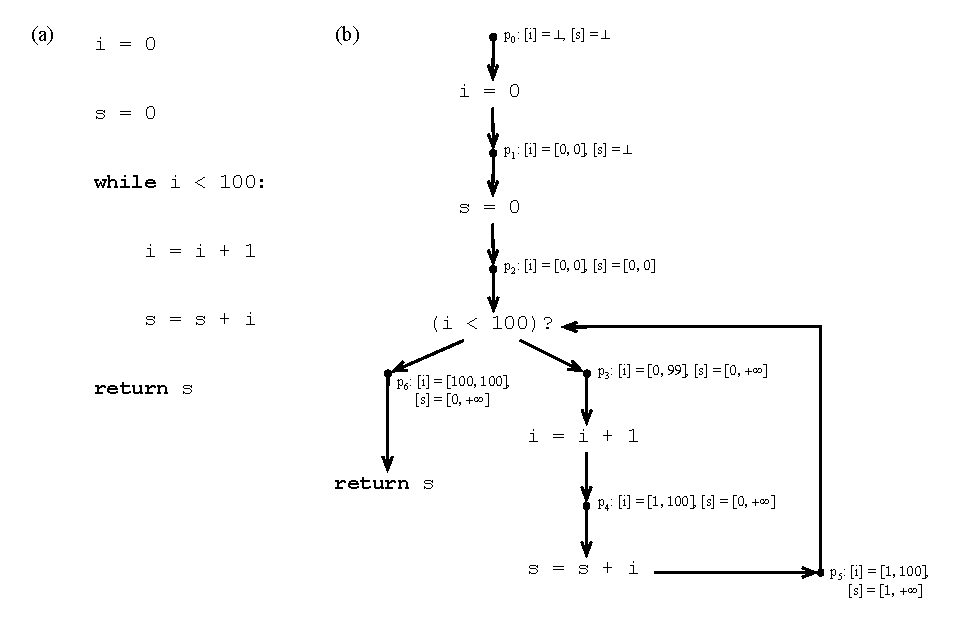
\includegraphics[width=\linewidth]{ProgramPoint}
\begin{minipage}[b]{0.2\textwidth}%
\begin{equation*}
\begin{array}[b]{l}
i=0;\\
s=0;\\
\whilett (i<100)\\
\quad i=i+1;\\
\quad s=s+i;\\
\returntt
\end{array}
\end{equation*}
\vspace{1cm}
\end{minipage}
\begin{minipage}[b]{0.4\textwidth}%
\tikzfigure{range}
\end{minipage}\hfill
\begin{minipage}[b]{0.35\textwidth}
\begin{equation*}
\begin{array}[b]{c|l|l}
\textit{prog. point} & [i] & [s]\\ \hline
0 & \top & \top\\
1 & [0,0] & \top\\
2 & [0,0] & [0,0]\\
3 & [0,100] & [0, +\infty[\\
4 & [100,100] & [0,+\infty[\\
5 & [0,99] & [0,+\infty[\\
6 & [0,100] & [0,+\infty[\\
7 & [0,100] & [0,+\infty[\\
\end{array}
\end{equation*}
\vspace{1cm}
\end{minipage}
\caption{An example of a dense data-flow analysis that finds the range of
possible values associated with each variable at each \progpoint.}
\label{fig:rangeAnalysis}
\end{figure}

The dense approach might keep more redundant information during the
data-flow analysis.
For instance, if we let $[v]^p$ denote the abstract state of variable
$v$ at \progpoint $p$, then we have that, in our example, $[i]^1 = [i]^2$,
$[s]^5 = [s]^6$ and $[i]^6 = [i]^7$.
This redundancy happens because some transfer functions are identities.
For instance, in range analysis, an instruction that neither defines nor uses any variable is associated with an identity transfer function.
The transfer function that updates the abstract state of $i$ at \progpoint $2$ is an identity.
Because the instruction immediately before $2$ does not add any new information to the abstract state of $i$, $[i]^2$ is updated with the information that flows directly from the predecessor point $1$.

The goal of sparse data-flow analysis is to shortcut the identity transfer functions, a task that we accomplish by grouping contiguous \progpoints bound to identities into larger regions.
Solving a data-flow analysis sparsely has many advantages over doing it densely: because we do not need to keep bitvectors associated with each \progpoint, the sparse solution tends to be more economical in terms of space and time.
Going back to our example, a given variable $v$ may be mapped to the same interval along many consecutive \progpoints.
Furthermore, if the information associated with a variable is invariant along its
entire live range, then we can bind this information to the variable itself.
In other words, we can replace all the constraint variables
$[v]^p$ by a single constraint variable $[v]$, for each variable $v$
and every $i\in \textrm{live}(v)$.
Not every data-flow problem can be easily solved sparsely; however, many of them can, as they fit into the family of PLV problems that we describe in the next section.

\subsection{Partitioned Lattice per Variable (PLV) Data-Flow Problems}
\label{sec:ssi:pereira:pvpPvl}

The class of non-relational data flow analysis problems we are interested in are the ones that bind information to pairs of program variables and \progpoints.
We design this class of problems as \emph{Partitioned Lattice per Variable} problems that we formally describe as follow.

\begin{definition}[PLV]
Let ${\cal V}=\{v_1,\dots,v_n\}$ be the set of program variables.
Let us consider, without loss of generality, a forward data-flow analysis.
This data-flow analysis can be written as an equation system that associates, with each \progpoint $p$, an element of a lattice ${\cal L}$, given by the equation $x^p = \bigwedge_{s \in \textit{preds}(p)} F^{s,p}(x^s)$, where: $x^p$ denotes the abstract state associated  with \progpoint $p$; for $s$ a control flow predecessor of $p$, $F^{s,p}$ is the transfer function from $s$ to $p$.
The analysis can alternatively be written\footnote{As far as we are concerned with finding its maximum solution. See for example Section~1.3.2 of~\cite{Nielson05}.} as a constraint system that binds to each \progpoint $p$ and each $s\in \textit{preds}(p)$ the equation $x^p = x^p \wedge  F^{s,p}(x^s)$ or, equivalently, the inequation $x^p \sqsubseteq  F^{s,p}(x^s)$.
The corresponding Maximum Fixed Point (MFP) problem is said to be a \emph{Partitioned Lattice per Variable Problem} iff $\cal L$ can be decomposed into the product of ${\cal L}_{v_1}\times \dots \times {\cal L}_{v_n}$ where each ${\cal L}_{v_i}$ is the lattice associated with program variable $v_i$. In other words $x^s$ can be writen as $([v_1]^s,\dots,[v_n]^s)$ where $[v]^s$ denotes the abstract state associated to variable $v$ and \progpoint $s$. $F^{s,p}$ can thus be decomposed into the product of $F^{s,p}_{v_1}\times \dots\times F^{s,p}_{v_n}$ and the constraint system decomposed into the inequalities $[v_i]^p\sqsubseteq  F^{s,p}_{v_i}([v_1]^s,\dots,[v_n]^s)$.
\end{definition}

Going back to range analysis, if we denote by $\cal I$ the lattice of integer intervals, then the overall lattice can be written as ${\cal L}={\cal I}^n$, where $n$ is the number of variables.
%
Note that the class of PLV problems include a smaller class of problems called {\em Partitioned Variable Problems} (PVP).
These analyses, which include live variables, reaching definitions and forward/backward printing, can be decomposed into a set of sparse data-flow problems -- usually one per variable -- each independent on the other.

\subsection{The Static Single Information Property}
\label{sec:ssi:pereira:singProp}

If the information associated with a variable is invariant along its
entire live range, then we can bind this information to the variable itself.
In other words, we can replace all the constraint variables
$[v]^p$ by a single constraint variable $[v]$, for each variable $v$
and every $p\in \textrm{live}(v)$. 
Consider the problem of range analysis again. There are two types of \splitpoints associated with non-identity transfer functions: definitions and conditionals:
(1) at the definition point of variable $v$, $F_v$ simplifies to a function that depends only on some $[u]$ where each $u$ is an argument of the instruction defining $v$;
(2) at the conditional tests that use a variable $v$, $F_v$ can be simplified to a function that uses $[v]$ and possibly other variables that appear in the test.
The other programs points are associated with an identity transfer function and can thus be ignored:  $[v]^p =[v]^p \wedge F_v^{s,p}([v_1]^s, \dots, [v_n]^s)$ simplifies to  $[v]^p = [v]^p \wedge [v]^p$ i.e. $[v]^p = [v]^p$. 
This gives the intuition on why a propagation engine along the def-use chains of a SSA-form program can be used to solve the constant propagation problem in an equivalent, yet ``sparser'', manner.
This also paves the way toward a formal definition of the Static Single Information property.

\begin{property}[SSI]
\label{pro:ssi}\textsc{Static Single Information:} Consider a forward (resp. backward) monotone PLV problem $E_\textit{dense}$ stated as a set of constraints $[v]^p \sqsubseteq F_v^{s,p}([v_1]^s,\dots,[v_n]^s)$ for every variable $v$, each \progpoint $p$, and each $s \in \textit{preds}(p)$ (resp. $s\in \textit{succs}(p)$).
A program representation fulfills the Static Single Information property iff:\begin{description}
\item {\bf [SPLIT]:} let $s$ be the unique predecessor (resp. successor) of a \progpoint where a variable $v$ is live and such that $F_v^{s,p}\neq \lambda x.\bot$ is non-trivial, i.e. is not the simple projection on ${\cal L}_v$, then $s$ should contain a definition (resp. last use) of $v$; 
Let $(Y_v^p)_{(v,p)\in \textit{variables}\times \textit{progPoints}}$ be a maximum solution to $E_\textit{dense}$. 
Each node $p$ that has several predecessors (resp. successors), and for which $F_v^{s,p}(Y_{v_1}^s,\dots,Y_{v_n}^s)$ has different values on its incoming edges $(s,p)$ (resp. outgoing edges $(p,s)$) should have a \phifun at the entry of $p$ (resp. \sigmafun at the exit of $p$) for $v$
as defined in Section~\ref{sub:ssi:split}.
\item {\bf [INFO]:} each program point $i$ such that $v\not\in \textrm{live-out}(i)$ (resp. $v\not\in \textrm{live-in}(i))$)  should be bound to an undefined  transfer function, i.e., $F_v^i=\lambda x.\bot$.
\item {\bf [LINK]:} each instruction \textit{inst} for which $F_v^{\textit{inst}}$ depends on some $[u]^s$ should contain an use (resp. def) of $u$ live-in (resp. live-out) at
\textit{inst}.
\item {\bf [VERSION]:} for each variable $v$, $\textrm{live}(v)$ is a connected component of the CFG.
\end{description}
\end{property}

These properties allows us to attach the information to variables, instead of \progpoints.
The {SPLIT} property forces the information related to a variable to be invariant along its entire live-range.
{INFO} forces this information to be irrelevant outside the live range of the variable.
The {LINK} property forces the def-use chains to reach the points where information is available for a transfer function to be evaluated.
The {VERSION} property provides an one-to-one mapping between variable names and live ranges.

We must split live ranges to provide the SSI properties.
If we split them between each pair of consecutive instructions, then we would automatically provide these properties, as the newly created variables
would be live at only one \progpoint.
However, this strategy would lead to the creation of many trivial program regions, and we would lose sparsity.
In Section~\ref{sec:building} we provide a sparser way to split live ranges that fit Property~\ref{pro:ssi}.
Possibly, we may have to extend the live-range of a variable to cover every \progpoint where the information is relevant.
We accomplish this last task by inserting into the program pseudo-uses and pseudo-definitions of this variable.

\subsection{Special instructions used to split live ranges}
\label{sub:ssi:split}

We perform live range splitting via special instructions: the \sigmafuns and parallel copies that, together with \phifuns, create new definitions of variables.
These notations are important elements of the propagation engine described in the section that follows.
In short, a \sigmafun (for a branch point) is the dual of a \phifun (for a join point), and a parallel copy is a copy that \emph{must} be done in parallel with another instruction.
Each of these special instructions, \phifun, \sigmafuns, and parallel copies split live ranges at different kinds of program points: interior nodes, branches and joins.

\emph{Interior nodes} are program points that have a unique predecessor and a unique successor.
At these points we perform live range splitting via copies.
If the program point already contains another instruction, then this copy \emph{must} be done \emph{in parallel} with the existing instruction.
The notation, \[\textit{inst} \ \parallel\  v_1=v'_1 \ \parallel\  \dots \ \parallel\  v_m=v'_m\] denotes $m$ copies $v_i=v'_i$ performed in parallel with
instruction \textit{inst}.
This means that all the uses of \textit{inst} plus all right-hand variables $v'_i$ are read simultaneously, then \textit{inst} is computed, then all definitions of \textit{inst} plus all left-hand variables $v_i$ are written simultaneously.
The null pointer analysis example of Figure~\ref{fig:ssi:nullAnalysis}(d), that we will explain later, uses parallel copies at nodes $l_4$ and $l_6$.


% need phi
We call {\em joins} the program points that have one successor and multiple predecessors.
For instance, two different definitions of the same variable $v$ might be associated with two different constants; hence, providing two different pieces of information about $v$.
To avoid that these definitions reach the same use of $v$ we merge them at the earliest program point where they meet.
We do it via our well-known \phifuns.

% need sigma
In backward analyses the information that emerges from different uses of a variable may reach the same {\em branch point}, which is a program point with a unique predecessor and multiple successors.
To ensure Property~\ref{pro:ssi}, the use that reaches the definition of a
variable must be unique, in the same way that in a SSA-form program the definition that reaches a use is unique.
We ensure this property via special instructions called \sigmafuns.
The \sigmafuns are the dual of \phifuns, performing a parallel assignment depending on the execution path taken.
The assignment \[(l^1:v_1^1, \ldots, l^q:v_1^q) = \sigma(v_1) \ \parallel\  \dots \ \parallel\  (l^1:v_m^1, \ldots, l^q:v_m^q) = \sigma(v_m)\] represents $m$ \sigmafuns that assign to each variable $v_i^j$ the value in $v_i$ if control flows into block $l^j$.
These assignments happen in parallel, i.e., the $m$ \sigmafuns encapsulate $m$ parallel copies.
Also, notice that variables live in different branch targets are given
different names by the \sigmafun that ends that basic block.
%TODO FAB: add reference to gated SSA, loop closed form etc.

\subsection{Propagating Information Forwardly and Backwardly}
\label{sec:ssi:pereira:engine}

Let us consider a unidirectional forward (resp. backward) PLV problem $E^{\textit{ssi}}_{\textit{dense}}$ stated as a set of equations $[v]^p \sqsubseteq  F_v^{s,p}([v_1]^s, \dots, [v_n]^s)$ (or equivalently $[v]^p = [v]^p \wedge    F_v^{s,p}([v_1]^s, \dots, [v_n]^s$) for every variable $v$, each \progpoint $p$, and each $s \in \textit{preds}(p)$ (resp. $s \in \textit{succs}(p)$). 
To simplify the discussion, any \phifun (resp. \sigmafun) is seen as a set of copies, one per predecessor (resp. successor), which leads to as many constraints.
In other words, a \phifun such as $p:a=\phi(a_1:l^1,\dots,a_m:l^m)$, gives us $n$ constraints such as $[a]^p \sqsubseteq  F_v^{l^j,p}([a_1]^{l^j}, \dots, [a_n]^{l^j})$, which usually simplifies into $[a]^p \sqsubseteq [a_j]^{l^j}$. This last can be written equivalently into the classical meet $[a]^p \sqsubseteq \bigwedge_{l^j \in \textit{preds}(p)} [a_j]^{l^j}$ used in Chapter~\ref{chapter:constant_propagation_is_easier}.
Similarly, a \sigmafun $(l^1:a_1,\dots,l^m:a_m)=\sigma(p:a)$ after \progpoint $p$ yields $n$ constraints such as $[a_j]^{l_j} \sqsubseteq  F_v^{p,l^j}([a_1]^p, \dots, [a_n]^p)$, which usually simplifies into $[a_j]^{l_j} \sqsubseteq [a]^p$.
Given a program that fulfills the SSI property for $E^{\textit{ssi}}_{\textit{dense}}$ and the set of transfer functions $F_v^s$, we show here how to build an equivalent sparse constrained system.  

\begin{definition}[SSI constrained system]
\label{def:ssi_eq}
Consider that a program in SSI form gives us a constraint system that associates with each variable $v$ the constraints $[v]^p \sqsubseteq  F_v^{s,p}([v_1]^s, \dots, [v_n]^s)$. We define a system of sparse equations $E^{\textit{ssi}}_{\textit{sparse}}$ as follows:

\begin{itemize}

\item For each instruction at a program point $i$ that defines (resp. uses) a variable $v$, we let $a \dots z$ be its set of used (resp. defined) variables. Because of the LINK property, $F^{s,p}_v$ (that we will denote $F^i_v$ from now) depends only on some $[a]^s \dots [z]^s$.
Thus, there exists a function $G^i_v$ defined as the restriction of $F^i_v$ on ${\cal L}_a\times \dots \times{\cal L}_z$, i.e. informally ``$G^i_v([a], \dots, [z]) = F^i_v([v_1],\dots, [v_n])$''.
% FAB: I do not like much this in,formal notation
\item The sparse constrained system associates with each variable $v$, and each definition (resp. use) point $i$ of $v$, the corresponding constraint $[v]  \sqsubseteq G_v^i([a], \ldots, [z])$ where $a,\dots, z$ are used (resp. defined) at $i$.
\end{itemize}

\end{definition}

The propagation engine discussed in Chapter~\ref{chapter:constant_propagation_is_easier} sends information forwardly along the def-use chains naturally formed by the SSA-form program.
If a given program fulfills the SSI property for a backward analysis, we can use a very similar propagation algorithm to communicate information backwardly.
Figure~\ref{alg:ssi:propback} shows a worklist algorithm that propagates information backwardly.
A slightly modified version of this algorithm, seen in Figure~\ref{alg:ssi:propforward} propagates information forwardly.
If necessary, these algorithms can be made control flow sensitive, like Algorithm~\ref{alg:constant_propagation_is_easier:propagation}. 


\def\1{\qquad}
\def\2{\1\1}
\def\3{\2\1}
\def\4{\2\2}
\def\5{\3\2}
\def\6{\4\2}
\def\7{\5\2}
\def\8{\6\2}
\def\9{\7\2}
\def\If{{\sf  if }}
\def\Let{{\sf  let }}
\def\Then{{\sf  then }}
\def\Else{{\sf  else}}
\def\Foreach{{\sf foreach }}
\def\For{{\sf for }}
\def\While{{\sf while }}


\newcommand\val[1]{[#1]}
\begin{algorithm}[t!]
\begin{tabular}{rl}
$_1$ & \textsf{function back\_propagate}(transfer\_functions $\cal G$)\\
$_2$ & \1$\var{worklist} = \emptyset$\\
$_3$ & \1\Foreach $\var{v} \in \textrm{vars}$: $\val{v}=\top$\\
$_4$ & \1\Foreach $\var{i} \in \textrm{insts}$: $\var{worklist}\ +\hspace{-0.3em}= i$\\
$_5$ & \1\While $\var{worklist}\neq \emptyset$:\\
$_6$ & \1\1 \Let $i \in \var{worklist}$; $\var{worklist}\ -\hspace{-0.3em}= \var{i}$\\
$_7$ & \1\1 \Foreach $v \in \var{i.uses}()$:\\
$_8$ & \1  \2  $\val{v}_{new} = \val{v} \wedge G_v^i(\val{\var{i.defs}()})$\\
$_9$ &  \1 \2  \If $\val{v} \neq \val{v}_{new}$: \\
$_{10}$& \1   \3 $\var{worklist}\ +\hspace{-0.3em}=\var{v.defs}()$\\
$_{11}$& \1   \3 $\val{v} = \val{v}_{new}$\\
\end{tabular}
\caption{\label{alg:ssi:propback} Backward propagation engine under SSI}
\end{algorithm}

\begin{algorithm}[t!]
\begin{tabular}{rl}
$_1$ & \textsf{function forward\_propagate}(transfer\_functions $\cal G$)\\
$_2$ & \1$\var{worklist} = \emptyset$\\
$_3$ & \1\Foreach $\var{v} \in \textrm{vars}$: $\val{v}=\top$\\
$_4$ & \1\Foreach $\var{i} \in \textrm{insts}$: $\var{worklist}\ +\hspace{-0.3em}= i$\\
$_5$ & \1\While $\var{worklist}\neq \emptyset$:\\
$_6$ & \1\1 \Let $i \in \var{worklist}$; $\var{worklist}\ -\hspace{-0.3em}= \var{i}$\\
$_7$ & \1\1 \Foreach $v \in \var{i.defs}()$:\\
$_8$ & \1  \2  $\val{v}_{new} =  G_v^i(\val{\var{i.uses}()})$\\
$_9$ &  \1 \2  \If $\val{v} \neq \val{v}_{new}$: \\
$_{10}$& \1   \3 $\var{worklist}\ +\hspace{-0.3em}=\var{v.uses}()$\\
$_{11}$& \1   \3 $\val{v} = \val{v}_{new}$\\
\end{tabular}
\caption{\label{alg:ssi:propforward} Forward propagation engine under SSI}
\end{algorithm}

Still we should outline a quite important subtlety that appears in line~8 of algorithms~\ref{alg:ssi:propback} and~\ref{alg:ssi:propforward}. $[v]$ appears (and has to) on the right hand side of the assignment for Algorithm~\ref{alg:ssi:propback} while it does not for Algorithm~\ref{alg:ssi:propforward}. This comes from the asymmetry of our SSI form that ensures (for practical purpose only as we will explain soon) the Static Single Assignment property but not the Static Single Use (SSU) property.
If we have several uses of the same variable, then the sparse backward constraint system will have several inequations -- one per variable use -- with the same left-hand-side.
Technically this is the reason why we manipulate a constraint system (system with inequations) and not an equation system as in Chapter~\ref{chapter:constant_propagation_is_easier}. Both systems can be solved~\footnote{in the ideal world with monotone framework and lattice of finite height} using a scheme known as \emph{chaotic iteration} such as the worklist algorithm we provide here. The slight and important difference for a constraint system as opposed to an equation system, is that one needs to meet $G_v^i(\dots)$ with the old value of $[v]$ to ensure the monotonicity of the consecutive values taken by $[v]$.
It would be still possible to enforce the SSU property, in addition to the SSA property, of our intermediate representation at the expenses of adding more \phifuns and \sigmafuns.
However, this guarantee is not necessary to every sparse analysis.
The dead-code elimination problem illustrates well this point:
for a program under SSA form, replacing $G_v^i$ in Algorithm~\ref{alg:ssi:propback} by ``\emph{i is a useful instruction or one of its definitions is marked as useful}'' leads to the standard SSA-based dead-code elimination algorithm.
The sparse constraint system does have several equations (one per variable use) for the same left-hand-side (one for each variable).
It is not necessary to enforce the SSU property in this instance of dead-code elimination, and doing so would lead to a less efficient solution, in terms of compilation time and memory consumption.
In other words, a code under SSA form fulfills the SSI property for dead-code elimination.


\subsection{Examples of sparse data-flow analyses}
\label{sub:ssi:examples}

As we have mentioned before, many data-flow analyses can be classified as PLV problems.
In this section we present some meaningful examples.

\paragraph{Range analysis revisited}
We start this section revising this chapter's initial example of data-flow analysis, given in Figure~\ref{fig:rangeAnalysis}.
A range analysis acquires information from either the points where variables are defined, or from the points where variables are tested.
In Figure~\ref{fig:rangeAnalysis-sparse} we know that $i$ must be bound to the interval $[0, 0]$ immediately after program point $l_1$.
Similarly, we know that this variable is upper bounded by 100 at entry of program point $l_4$, due to the conditional test that happens before.
Therefore, in order to achieve the SSI property, we should split the live ranges of variables at their definition points, or at the conditionals where they are used.
Figure~\ref{fig:rangeAnalysis-sparse}(a) shows the original example after live range splitting.
In order to ensure the SSI property in this example, the live range of variable $i$ must be split at its definition, and at the conditional test.
The live range of $s$, on the other hand, must be split only at its definition point, as it is not used in the conditional.
Splitting at conditionals is done via \sigmafuns.
The representation that we obtain by splitting live ranges at definitions and conditionals is called the Extended Static Single Assignment (e-SSA) form.
Figure~\ref{fig:rangeAnalysis-sparse}(b) shows the result that we obtain by running the range analysis on this intermediate representation.
This solution assigns to each variable a unique range interval.

\begin{figure}[t!]
\centering
\tikzfigure{range-ssi}\hfill
\begin{minipage}[b]{0.4\textwidth}
\begin{equation*}
\begin{array}[b]{ll}
[i_1] = [i_1] \cup [0,0] &= [0,0]\\

[s_1] = [s_1] \cup [0,0] &= [0,0]\\

[i_2] = [i_2] \cup [i_1] \cup [i_4] &= [0,100]\\

[s_2] = [s_2] \cup [s_1] \cup [s_3] &= [0,+\infty[\\

[i_3] = [i_3] \cup \left([i_2] \cap \left]-\infty,99\right]\right) &= [0,99]\\

[i_4] = [i_4] \cup \left([i_3] + 1\right) &= [1,100]\\ 

[s_3] = [s_3] \cup \left([s_2] + [i_4]\right) &= [1,+\infty[\\~\\\\
\end{array}
\end{equation*}
\end{minipage}
\caption{(a) The example from Figure~\ref{fig:rangeAnalysis} after live range splitting.
(b) A solution to this instance of the range analysis problem.}
\label{fig:rangeAnalysis-sparse}
% TODO FAB rappeler l'example de la fig 1.1. 
%TODO FAB: add the equations in (b): [i_1]=[i_0] \cups [i_3]; [i_2]=[i_1] \cap [-\infty,99]; [i_3]=[i_2]+1; [s_1]=[s_0]\cups[s_2]; [s_2]=[s_1]+[i_3] (widening required here)
\end{figure}



\paragraph{Class Inference} Some dynamically typed languages, such as Python, Java\-Scrip, Ruby or Lua, represent objects as tables containing methods and fields.
It is possible to improve the execution of programs written in these languages if we can replace these simple tables by actual classes with virtual tables.
A class inference engine tries to assign a class to a variable $v$ based on the ways that $v$ is defined and used.
The Python program in Figure~\ref{fig:classInference}(a) illustrates this optimization.
Our objective is to infer the correct suite of methods for each object bound to variable $v$.
Figure~\ref{fig:classInference}(b) shows the control-flow graph of the program, and Figure~\ref{fig:classInference}(c) shows the results of a dense implementation of this analysis.
Because type inference is a backward analysis that extracts information from use sites, we split live ranges at these program points, and rely on \sigmafuns to merge them back, as we see in Figure~\ref{fig:classInference}(e).
The use-def chains that we derive from the program representation lead naturally to a constraint system, which we show in Figure~\ref{fig:classInference}(f), where $[v_j]$ denotes the set of methods associated with variable $v_j$.
A fix-point to this constraint system is a solution to our data-flow problem.
This instance of class inference is a Partitioned Variable Problem~(PVP)~\footnote{Actually class inference is no more a PVP as soon as we want to propagate the information through copies.}, because the data-flow information associated with a variable $v$ can be computed independently from the other variables.

\begin{figure}[t!]
%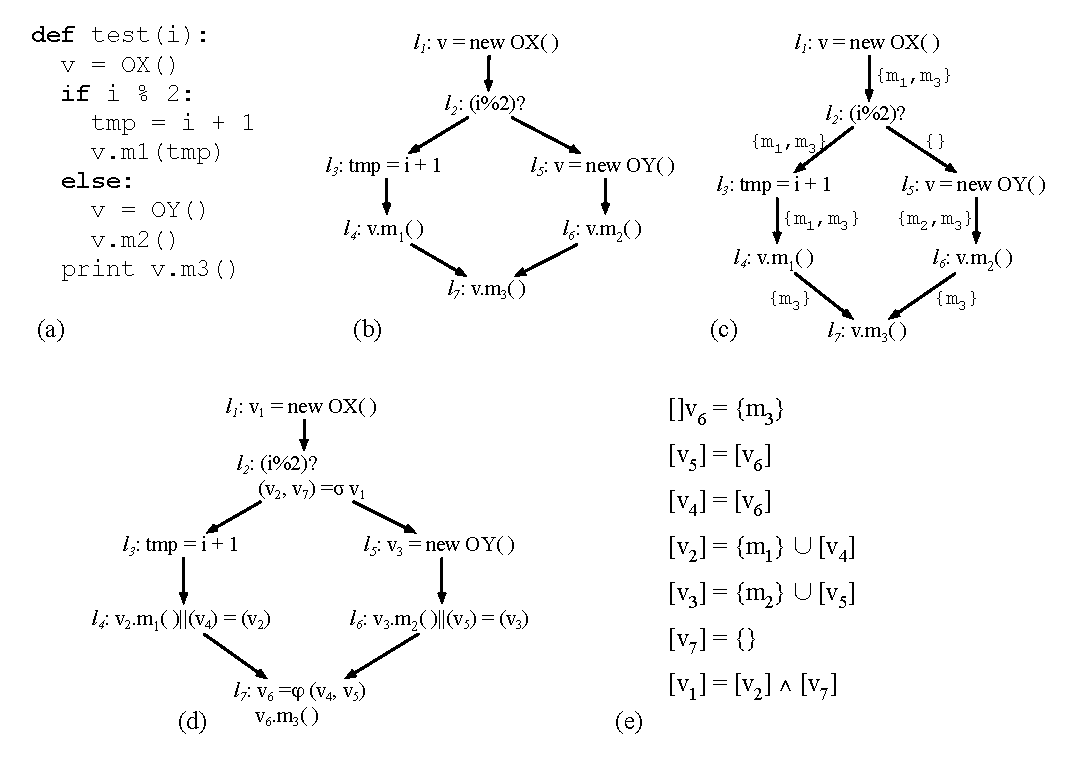
\includegraphics[width=\linewidth]{classInference}
%\tikzfigure{class-inference}
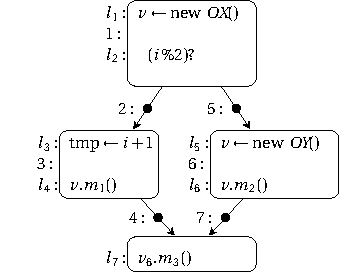
\includegraphics[scale=0.85]{tikz/class-inference}
\hfill
%\tikzfigure{class-inference-ssi}
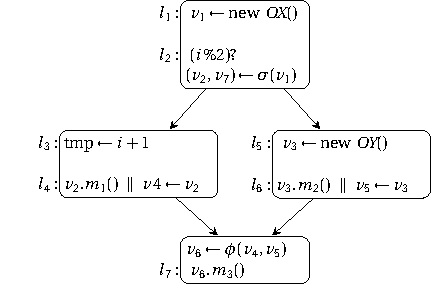
\includegraphics[scale=0.85]{tikz/class-inference-ssi}\\
~\\
\begin{minipage}[b]{0.35\textwidth}
\begin{equation*}
\begin{array}[b]{c|l}
\textit{prog. point} & [v]\\ \hline
1 & \{m_1, m_3\}\\
2 & \{m_1, m_3\}\\
3 & \{m_1, m_3\}\\
4 & \{m_3\}\\
5 & \top\\
6 & \{m_2, m_3\}\\
7 & \{m_3\}
\end{array}
\end{equation*}
\end{minipage}\hfill
\begin{minipage}[b]{0.5\textwidth}
$$
\begin{array}[b]{lll}
[v_6] &=& [v_6] \wedge \{ m_3 \} = \{ m_3 \}\\

[v_5] &=& [v_5] \wedge [v_6] = \{m_3\}\\

[v_4] &=& [v_4] \wedge [v_6] = \{m_3\}\\

[v_2] &=& [v_2] \wedge \left(\{m_1\} \wedge [v_4]\right) = \{m_1,m_3\}\\

[v_3] &=& [v_3] \wedge \left(\{m_2\} \wedge [v_4]\right) = \{m_2,m_3\}\\

[v_1] &=& [v_1] \wedge [v_2] = \{m_1,m_3\}\\

[v_1] &=& [v_1] \wedge [v_7] = \{m_1,m_3\}
\end{array}
$$
\end{minipage}
\caption{Class inference analysis as an example of backward data-flow analysis that takes information from the uses of variables.}
\label{fig:classInference}
%TODO FAB: virer les new dans la figure. Virer les points de programme qui ne servent à rien en (d) (car erreur sur l7)
\end{figure}


\paragraph{Null pointer analysis} The objective of null pointer analysis is to determine which references may hold null values.
This analysis allows compilers to remove redundant null-exception tests and helps developers to find null pointer dereferences.
Figure~\ref{fig:ssi:nullAnalysis} illustrates this analysis.
Because information is both produced at definition but also at use sites, we split live ranges after each variable is used, as we show in Figure~\ref{fig:ssi:nullAnalysis}(b).
For instance, we know that $v_2$ cannot be null and hence the call $v_2.m()$ cannot result in a null pointer dereference exception, otherwise an exception would have been thrown during the invocation $v_1.m()$.
On the other hand, in Figure~\ref{fig:ssi:nullAnalysis}(c) we notice that the state of $v_4$ is the meet of the state of $v_3$, definitely not-null, and the state of $v_1$, possibly null, and we must conservatively assume that $v_4$ may be null.


\begin{figure}[t!]
\hspace{-1cm}\tikzfigure{null-pointer}
\hspace{-0.4cm}\tikzfigure{null-pointer-ssi}
\begin{minipage}[b]{0.24\textwidth}
\begin{equation*}
\begin{array}{l}
[v_1] = [v_1] \wedge 0 = 0\\

[v_2] = [v_2] \wedge \nonnull = \nonnull\\

[v_3] = [v_3] \wedge \nonnull = \nonnull\\

[v_4] = [v_4] \wedge \left([v_3] \wedge [v_1]\right) = 0
\end{array}
\end{equation*}
\vspace{1cm}
\end{minipage}
\caption{Null pointer analysis as an example of forward data-flow analysis that takes information from the definitions and uses of variables ($0$ represents the fact that the pointer is possibly null, $\nonnull$ if it cannot be).} \label{fig:ssi:nullAnalysis}
%TODO: add [v4]=possibly null
\end{figure}


\section{Construction and Destruction of the Intermediate Program Representation}
\label{sec:building}
\def\Sdown{\downarrow}
\def\Sup{\uparrow}
\def\SS{{\cal P}}
\def\Out{\textrm{Out}}
\def\In{\textrm{In}}
\def\Defs{\textrm{Defs}}
\def\Def{\textrm{Def}}
\def\Uses{\textrm{Uses}}

In the previous section we have seen how the static single information
property gives the compiler the opportunity to solve a data-flow problem sparsely.
However, we have not yet seen how to convert a program to a format that provides the SSI property.
This is a task that we address in this section, via the three-steps algorithm from Section~\ref{sub:ssi:ssify}.

\subsection{Splitting strategy}
A {\em live range splitting strategy} \
$\SS_v = I_\uparrow \cup I_\downarrow$ over a variable $v$ consists of a set
of ``oriented'' program points.
We let $I_\downarrow$ denote a set of points $i$ with forward direction.
Similarly, we let $I_\uparrow$ denote a set of points $i$ with backward
direction.
The live-range of $v$ must be split at least at every point in $\SS_v$.
Going back to the examples from Section~\ref{sub:ssi:examples}, we have the live range splitting strategies enumerated below.
The list in Figure~\ref{fig:splittingSt} gives further examples of live range splitting strategies. Corresponding references are given in the last section of this chapter.

\begin{itemize}
\item Range analysis, is a forward analysis that takes information from points where variables are defined, and conditional tests that use these variables.
For instance, in Figure~\ref{fig:rangeAnalysis-sparse}, we have that $\SS_{i} = \{l_1, \Out(l_3), l_4\}_\downarrow$ where $\Out(l_i)$ denotes the exit of $l_i$ (i.e. the \progpoint immediately after $l_i$), and that $\SS_{s}=\{l_2, l_5\}_\downarrow$.

\item Class inference is a backward analysis that takes information from the uses of variables; thus, for each variable, the live-range splitting strategy is characterized by the set $\textit{Uses}_\uparrow$ where $\textit{Uses}$ is the set of use points.
For instance, in Figure~\ref{fig:classInference}(d), we have that
$\SS_{v} = \{l_4, l_6,l_7\}_\uparrow$.


\item Null pointer analysis takes information from definitions and uses and propagates this information forwardly.
For instance, in Figure~\ref{fig:ssi:nullAnalysis}, we have that
$\SS_{v} = \{l_1, l_2, l_3, l_4\}_\downarrow$.
\end{itemize}

\begin{figure}[t!]
\begin{center}
\begin{small}
\renewcommand\arraystretch{1.4}
\begin{tabular}{| c | c |} \hline
{\bf Client} & {\bf Splitting strategy $\SS$} \\ \hline 
Alias analysis, reaching definitions & $\textit{Defs}_\downarrow$ \\ 
cond. constant propagation &  \\ \hline  
Partial Redundancy Elimination & $\textit{Defs}_\downarrow \bigcup \textit{LastUses}_\uparrow$ \\ \hline 
ABCD, taint analysis,  & $\textit{Defs}_\downarrow \bigcup \textit{\Out(Conds)}_\downarrow$ \\ 
range analysis & \\ \hline 
Stephenson's bitwidth analysis & $\textit{Defs}_\downarrow \bigcup \textit{\Out(Conds)}_\downarrow \bigcup \textit{Uses}_\uparrow$  \\ \hline 
Mahlke's bitwidth analysis & $\textit{Defs}_\downarrow \bigcup \textit{Uses}_\uparrow$  \\ \hline 
An's type inference, Class inference & $\textit{Uses}_\uparrow$ \\ \hline 
Hochstadt's type inference & $\textit{Uses}_\uparrow \bigcup \textit{\Out(Conds)}_\uparrow$ \\ \hline 
Null-pointer analysis & $\textit{Defs}_\downarrow \bigcup\textit{Uses}_\downarrow$ \\ \hline
\end{tabular} \end{small} 
\caption{Live range splitting strategies for different data-flow analyses.
$\textit{Defs}$ (resp. $\textit{Uses}$) denotes the set of instructions that define (resp. use) the variable. $\textit{Conds}$ denotes the set of instructions that apply a conditional test on a variable; $\Out(\textit{Conds})$ denotes the exits of the corresponding basic blocks; $\textit{LastUses}$ denotes the set of instructions where a variable is used, and after which it is no longer live.}
\label{fig:splittingSt} \end{center} \end{figure}

\def\SSIfy{\textsf{SSIfy}}

The algorithm \textsf{\SSIfy} in Figure~\ref{fig:SSIfy} implements a
live range splitting strategy in three steps.
Firstly, it splits live ranges, inserting new definitions of variables into the
program code.
Secondly, it renames these newly created definitions; hence, ensuring that
the live ranges of two different re-definitions of the same variable do not
overlap.
Finally, it removes dead and non-initialized definitions from the program code.
We describe each of these phases in the rest of this section.

\begin{figure}[htbp]
\begin{tabular}{rl}
$_1$& \textsf{function \SSIfy}(var \var{v}, Splitting\_Strategy $\SS_v$)\\
$_2$& \1\textsf{split}($v$, $\SS_v$)\\
$_3$& \1\textsf{rename}($v$)\\
$_4$& \1\textsf{clean}($v$)\\
\end{tabular}
\caption{\label{fig:SSIfy} Split the live ranges of $v$ to convert it to SSI form}
\end{figure}

\subsection{Splitting live ranges}
\label{sub:ssi:ssify}

In order to implement $\SS_v$ we must split the live ranges of $v$ at each
program point listed by $\SS_v$.
However, these points are not the only ones where splitting might be
necessary.
As we have pointed out in Section~\ref{sub:ssi:split}, we might have, for the same original variable, many different sources of information reaching a common program point.
For instance, in Figure~\ref{fig:rangeAnalysis}, there exist two definitions of variable $i$, e.g., $l_1$ and $l_4$, that reach the use of $i$ at $l_3$.
The information that flows forward from $l_1$ and $l_4$ collides at $l_3$, the loop entry.
Hence the live-range of $i$ has to be split immediately before $l_3$ -- at $\In(l_3)$ --, leading,
in our example, to a new definition $i_1$.
In general, the set of \progpoints where information collides can be easily
characterized by the notion of join sets and iterated dominance frontier ($\textit{DF}^+$) seen in Chapter~\ref{chapter:alternative_ssa_construction_algorithms}.
Similarly, split sets created by the backward propagation of information can
be over-approximated by the notion of {\em iterated post-dominance
frontier} ($\textit{pDF}^+$), which is the dual of
$\textit{DF}^+$.
That is, the post-dominance frontier is the dominance frontier in a CFG where
direction of edges have been reversed. Note that, just as the notion of dominance requires the existence of a unique entry node that can reach every CFG node, the notion of post dominance requires the existence of a unique exit node reachable by any CFG node. For control-flow graphs that contain several exit nodes or loops with no exit, we can ensure the single-exit property by creating a dummy common exit node and inserting some never-taken exit edges into the program.

\begin{figure}[t!]
\begin{small}
\begin{tabular}{rl}
$_1$&{\sf function split}(var \var{v}, Splitting\_Strategy
$\SS_v = I_\downarrow \cup I_\uparrow$)\\
$_2$&\1 ``compute the set of split nodes"\\
$_3$&\1$S_\uparrow = \emptyset$\\
$_4$&\1\Foreach $i \in I_\uparrow$:\\
$_5$&\1\1 \If $i.\textrm{is\_join}$:\\
$_6$&\1  \2 \Foreach $e\in \textit{incoming\_edges}(i)$:\\
$_7$&\1     \3  $S_\uparrow = S_\uparrow \bigcup \Out(pDF^+(e))$\\
$_8$&\1\1 \Else:\\
$_9$&\1  \2 $S_\uparrow = S_\uparrow \bigcup \Out(pDF^+(i))$\\
$_{10}$&\1$S_\downarrow = \emptyset$\\
$_{11}$&\1\Foreach $i \in S_\uparrow \bigcup \Defs(v) \bigcup I_\downarrow$:\\
$_{12}$&\1\1 \If $i.\textrm{is\_branch}$:\\
$_{13}$&\1  \2 \Foreach $e \in \textit{outgoing\_edges}(i)$\\
$_{14}$&\1      \3 $S_\downarrow = S_\downarrow \bigcup \In(DF^+(e))$\\
$_{15}$&\1\1 \Else:\\
$_{16}$&\1  \2 $S_\downarrow = S_\downarrow \bigcup \In(DF^+(i))$\\
$_{17}$&\1$S = \SS_v \bigcup S_\uparrow \bigcup S_\downarrow$\\
$_{18}$&\1 ``Split live range of $v$ by inserting $\phi$, $\sigma$, and copies"\\
$_{19}$&\1\Foreach  $i \in S$:\\
$_{20}$&\1\1 \If $i$ does not already contain any definition of $v$:\\
$_{21}$&\1   \2  \If $i.\textrm{is\_join}$: insert ``$v=\phi(v,...,v)$" at $i$\\
$_{22}$&\1   \2  \Else \If $i.\textrm{is\_branch}$: insert ``$(v,...,v)= \sigma(v)$" at  $i$\\
$_{23}$&\1   \2 else: insert a copy ``$v=v$" at $i$\\
\end{tabular}
\caption{\label{fig:Spliting} Live range splitting. We use $\In(l)$ to denote a program point immediately before $l$, and $\Out(l)$ to denote a program point immediately after $l$.} 
\end{small}
\end{figure}

Figure~\ref{fig:Spliting} shows the algorithm that we use to create new
definitions of variables.
This algorithm has three main phases.
First, in lines 3-9 we create new definitions to split the live ranges
of variables due to backward collisions of information.
These new definitions are created at the iterated post-dominance
frontier of points that originate information.
If a program point is a join node, then each of its predecessors
will contain the live range of a different definition of $v$, as we ensure
in lines 6-7 of our algorithm.
Notice that these new definitions are not placed parallel to an instruction,
but in the region immediately after it, which we denote by $\Out(\dots)$.
In lines 10-16 we perform the inverse operation: we create new definitions of
variables due to the forward collision of information.
Our starting points $S_\downarrow$, in this case, include also the original definitions of
$v$, as we see in line 11, because we want to stay in SSA form in order to
have access to a fast liveness check as described in Chapter~\ref{chapter:ssa_tells_nothing_of_liveness}.
Finally, in lines 17-23 we actually insert the new definitions of $v$.
These new definitions might be created by $\sigma$ functions (due to $\SS_v$ or
to the splitting in lines 3-9); by \phifuns (due to $\SS_v$ or to the
splitting in lines 10-16); or by parallel copies.

\begin{figure}[t!]
\begin{small}
\begin{tabular}{rl}
$_{1}$&{\sf function rename(var $v$)}\\
$_{2}$&\1 ``Compute use-def \& def-use chains"\\
$_{3}$&\1 ``We consider here that $\textsf{stack.peek}()=\bot$ if
{\sf stack.isempty()},\\
$_{4}$&\1~~~and that $def(\bot)=entry$"\\
$_{5}$&\1$stack = \emptyset$\\
$_{6}$&\1\Foreach CFG node $n$ in dominance order:\\
$_{7}$&\1\1 \If exists $v =\phi(v: l^1, \ldots, v: l^q)$ in $\In(n)$:\\
$_{8}$&\1  \2 $\textsf{stack.set\_def}(v =\phi(v: l^1, \ldots, v: l^q))$\\
$_{9}$&\1\1 \Foreach instruction $u$ in $n$ that uses $v$:\\
$_{10}$&\1  \2 $\textsf{stack.set\_use}(u)$\\
$_{11}$&\1\1 \If exists instruction $d$ in $n$ that defines $v$:\\
$_{12}$&\1  \2 $\textsf{stack.set\_def}(d)$\\
$_{13}$&\1\1 \Foreach instruction $(\ldots) =\sigma(v)$ in $\Out(n)$:\\
$_{14}$&\1  \2 $\textsf{stack.set\_use}((\ldots) =\sigma(v))$\\
$_{15}$&\1\1 \If exists $(v: l^1, \ldots, v: l^q) =\sigma(v)$ in $\Out(n)$:\\
$_{16}$&\1  \2 \Foreach $v: l^i = v$ in $(v: l^1, \ldots, v: l^q) =\sigma(v)$:\\
$_{17}$&\1     \3 $\textsf{stack.set\_def}(v: l^i = v)$\\
$_{18}$&\1\1 \Foreach $m$ in $successors(n)$:\\
$_{19}$&\1  \2 \If exists $v =\phi(\dots, v:l^n, \ldots)$ in $\In(m)$:\\
$_{20}$&\1     \3 $\textsf{stack.set\_use}(v = v: l^n)$\\  
\end{tabular}

\begin{tabular}{rl}
$_{21}$&\textsf{function stack.set\_use(instruction \var{inst})}:\\
$_{22}$&\1\While $def(\textsf{stack.peek()})$ does not dominate inst: \textsf{stack.pop()}\\
$_{23}$&\1$v_i = \textsf{stack.peek()}$\\
$_{24}$&\1replace the uses of $v$ by $v_i$ in inst\\
$_{25}$&\1\If $v_i\neq \bot$: set $\Uses(v_i)=\Uses(v_i) \bigcup$ inst
\end{tabular}

\begin{tabular}{rl}
$_{26}$&\textsf{function stack.set\_def}(instruction inst):\\
$_{27}$&\1let $v_i$ be a fresh version of $v$\\
$_{28}$&\1replace the defs of $v$ by $v_i$ in inst\\
$_{29}$&\1set $\Def(v_i)=$ inst\\
$_{30}$&\1$\textsf{stack.push}(v_i)$
\end{tabular}
\end{small}
\caption{\label{fig:Rename} Versioning} 
\end{figure}

\subsection{Variable Renaming}
The algorithm in Figure~\ref{fig:Rename} builds def-use and use-def chains
for a program after live range splitting.
This algorithm is similar to the classic algorithm used to rename variables
during the SSA construction that we saw in Chapter~\ref{chapter:classical_construction_algorithm}.
To rename a variable $v$ we traverse the program's dominance tree, from top to
bottom, stacking each new definition of $v$ that we find.
The definition currently on the top of the stack is used to replace all the
uses of $v$ that we find during the traversal.
If the stack is empty, this means that the variable is not defined at this point.
The renaming process replaces the uses of undefined variables by $\bot$ (line~3). 
We have two methods, \textsf{stack.set\_use} and \textsf{stack.set\_def} that build
the chains of relations between variables.
Notice that sometimes we must rename a single use inside a \phifun,
as in lines~19-20 of the algorithm.
For simplicity we consider this single use as a simple
assignment when calling \textsf{stack.set\_use}, as one can see in line 20.
Similarly, if we must rename a single definition inside a \sigmafun, then we treat it as a simple assignment, like we do in lines 15-16 of the algorithm.

\begin{figure}[t!]
\begin{small}
\begin{tabular}{rl}
$_{1}$ & \textsf{clean}(var $v$)\\
$_{2}$ & \1 \Let web = $\{ v_i | v_i \textrm{ is a version of } v \}$\\
$_{3}$ & \1 \Let defined = $\emptyset$\\
$_{4}$ & \1 \Let active = \{ $\var{inst} \ | \var{inst}$ actual instruction and $\textrm{web}\cap \var{inst}.\textrm{defs}  \neq \emptyset \}$\\
$_{5}$ & \1 \While $\exists \var{inst} \in \textrm{active}$ s.t. $\textrm{web}\cap\var{inst}.\textrm{defs} \backslash  \textrm{defined}\neq\emptyset$:\\
$_{6}$ & \1  \1 \Foreach $v_i \in \textrm{web}\cap\var{inst}.\textrm{defs} \backslash \textrm{defined}$: \\
$_{7}$ & \1     \2 active = active $\cup$ $\Uses(v_i)$ \\
$_{8}$ & \1     \2 defined = defined $\cup$ $\{ v_i \}$ \\
$_{9}$ & \1 \Let used = $\emptyset$\\
$_{10}$ & \1 \Let active = \{ $\var{inst} \ | \var{inst}$ actual instruction and $\textrm{web}\cap\var{inst}.\textrm{uses} \neq \emptyset \}$\\
$_{11}$ & \1 \While $\exists \var{inst} \in \textrm{active}$ s.t. $\var{inst}.\textrm{uses} \backslash  \textrm{used}\neq\emptyset$:\\
$_{12}$ & \1  \1 \Foreach $v_i \in \textrm{web}\cap\var{inst}.\textrm{uses} \backslash \textrm{used}$: \\
$_{13}$ & \1     \2 active = active $\cup$ $\Def(v_i)$ \\
$_{14}$ & \1     \2 used = used $\cup$ $\{ v_i \}$ \\
$_{15}$ & \1 \Let live = defined $\cap$ used\\
$_{16}$ & \1 \Foreach non actual $\var{inst} \in \Def(web)$:\\
$_{17}$ & \1  \1 \Foreach $v_i$ operand of \var{inst} s.t. $v_i \notin \textrm{live}$:\\
$_{18}$ & \1             \4 replace $v_i$ by $\bot$\\
$_{19}$ & \1  \1 \If $\var{inst}.\textrm{defs}=\{\bot\}$ or $\var{inst}.\textrm{uses}=\{\bot\}$\\
$_{20}$ & \1  \2 remove \var{inst}\\
\end{tabular}
\end{small}
\caption{\label{fig:clean} Dead and undefined code elimination. Original instructions not inserted by \textsf{split} are called \emph{actual} instruction. We let {\em inst}.defs denote the set of variable(s) defined by {\em inst}, and {\em inst}.uses denote the set of variables used by {\em inst}.}
\end{figure}

\subsection{Dead and Undefined Code Elimination}

Just as Algorithm~\ref{alg:classical_construction_algorithm:pruning}, the algorithm in Figure~\ref{fig:clean} eliminates \phifuns and parallel copies that define variables not actually used in the code. By symmetry, it also eliminates \sigmafuns  and parallel copies  that use variables not actually defined in the code.
We mean by ``actual'' instructions, those instructions that already existed in the program before we transformed it with \textsf{split}.
In line~3 we let ``web'' be the set of versions of $v$, so as to restrict the cleaning process to variable~$v$, as we see in lines~4-6 and lines~10-12.
The set ``active'' is initialized to actual instructions in line~4.
Then, during the loop in lines~5-8 we add to active \phifuns, \sigmafuns, and copies that can reach actual definitions through use-def chains.
The corresponding version of $v$ is then marked as \emph{defined} (line~8).
The next loop, in lines 11-14 performs a similar process, this time to add to the active set instructions that can reach actual uses through def-use chains.
The corresponding version of $v$ is then marked as \emph{used} (line~14).
Each non live variable (see line~15), i.e. either undefined or dead (non used) is replaced by $\bot$ in all $\phi$, $\sigma$, or copy functions where it appears in.
This is done by lines~15-18.
Finally every useless $\phi$, $\sigma$, or copy functions are removed by lines~19-20. 

\subsection{Implementation Details}
\label{sub:special}

%TODO: we need to explain how to get rid of copies in parallel with another instruction here.
\paragraph{Implementing \sigmafuns: }
The most straightforward way to implement \sigmafuns, in a compiler that already supports the SSA form, is to represent them by \phifuns.
In this case, the \sigmafuns can be implemented as single arity \phifuns.
As an example, Figure~\ref{fig:sigImpl}(a) shows how we would represent the \sigmafuns of Figure~\ref{fig:classInference}(d). 
If $l$ is a branch point with $n$ successors that would contain a \sigmafun $(l^1:v_1, \ldots, l^n:v_n) =\sigma(v)$, then, for each successor $l^j$ of $l$, we insert at the beginning of $l^j$ an instruction $v_j = \phi(l^j:v)$.
Notice that it is possible that $l^j$ already contains a \phifun for $v$.
This case happens when the control flow edge $l \rightarrow l^j$ is {\em critical}.
A critical edge links a basic block with several successors to a basic block with several predecessors.
If $l^j$ already contains a \phifun $v' = \phi(\ldots, v_j, \ldots)$, then we rename $v_j$ to $v$.

\begin{figure}[t!]
\hspace{-1.2cm}\tikzfigure{class-inference-ssi-out-1}\hspace{-0.6cm}
\tikzfigure{class-inference-ssi-out-2}
\caption{(a) implementing \sigmafuns via single arity \phifuns; (b) getting rid of copies and \sigmafuns.}
\label{fig:sigImpl}
\end{figure}

\paragraph{SSI Destruction: }
Traditional instruction sets do not provide \phifuns nor \sigmafuns.
Thus, before producing an executable program, the compiler must implement these instructions.
We have already seen in Chapter~\ref{chapter:classical_construction_algorithm} how to replace \phifuns with actual assembly instructions; however, now we must also replace \sigmafuns and parallel copies.
A simple way to eliminate all the \sigmafuns and parallel copies is via copy-propagation.
In this case, we copy-propagate the variables that these special instructions define.
As an example, Figure~\ref{fig:sigImpl}(b) shows the result of copy folding applied on Figure~\ref{fig:sigImpl}(a).

\section{Further Reading}

The monotone data-flow framework is an old ally of compiler writers.
Since the work of pionners like Prosser~\cite{Prosser59}, Allen~\cite{Allen70,Allen76}, Kildall~\cite{Kildall77} and Hecht~\cite{Hecht77}, data-flow analyses such as reaching definitions, available expressions and liveness analysis have made their way into the implementation of virtually every important compiler.
Many compiler textbooks describes the theoretic basis of the notions of lattice, monotone data-flow framework and fixed points.
For a comprehensive overview of these concepts, including algorithms and formal proofs, we refer the interested reader to Nielson {\em et al.}'s book~\cite{Nielson05} on static program analysis.

The original description of the intermediate program representation known as Static Single Information form was given by Ananian in his Master's thesis~\cite{Ananian99}.
The notation for \sigmafuns that we use in this chapter was borrowed from Ananian's work.
The SSI program representation was subsequently revisited by Jeremy Singer in his PhD thesis~\cite{Singer06}.
Singer proposed new algorithms to convert programs to SSI form, and also showed how this program representation could be used to handle truly bidirectional data-flow analyses.
We did not discuss bidirectional data-flow problems, but the interested reader can find examples of such analyses in Khedker {\em et al.}'s work~\cite{Khedker99}.
Working on top of Ananian's and Singer's work, Boissinot {\em et al.}~\cite{BoissinotBDR12} have proposed a new algorithm to convert a program to SSI form.
Boissinot {\em et al.} have also separated the SSI program representation in two flavors, which they call {\em weak} and {\em strong}.
Tavares {\em et al.}~\cite{Tavares11b} have extended the literature on SSI representations, defining building algorithms and giving formal proofs that these algorithms are correct.
The presentation that we use in this chapter is mostly based on Tavares {\em et
al.}'s work.

There exist other intermediate program representations that, like the SSI form, make it possible to solve some data-flow problems sparsely.
Well-known among these representations is the {\em Extended Static Single Assignment} form, introduced by Bodik {\em et al.} to provide a fast algorithm to eliminate array bound checks in the context of a JIT compiler~\cite{Bodik00}.
Another important representation, which supports data-flow analyses that acquire information at use sites, is the \emph{Static Single Use} form (SSU).
As uses and definitions are not fully symmetric (the live-range can ``traverse'' a use while it cannot traverse a definition) there exists different variants of SSU (eg.~\cite{Plevyak96,George03-IXP,Lo98_registerPromotion}).
For instance, the ``strict'' SSU form enforces that each definition reaches a
single use, whereas SSI and other variations of SSU allow two consecutive uses
of a variable on the same path.
All these program representations are very effective, having seen use in a number of implementations of flow analyses; however, they only fit specific data-flow problems.

The notion of {\em Partitioned Variable Problem} (PVP) was introduced by Zadeck, in his PhD dissertation~\cite{Zadeck84}.
Zadeck proposed fast ways to build data-structures that allow one to solve these problems efficiently.
He also discussed a number of data-flow analyses that are partitioned variable problems.
There are data-flow analyses that do not meet the Partitioned Lattice per Variable property.
Noticeable examples include abstract interpretation problems on relational domains, such as Polyhedrons~\cite{Cousot78}, Octagons~\cite{Mine06} and Pentagons~\cite{Logozzo08}.
%This domain binds variables together in constraints such as $x + y \leq c$, where $c$ is an integer, and $x, y$ are program variables.

In terms of data-structures, the first, and best known method proposed to support sparse data-flow analyses is Choi {\em et al.}'s {\em Sparse Evaluation Graph} (SEG)~\cite{Choi91}.
The nodes of this graph represent program regions where information produced by the data-flow analysis might change.
Choi {\em et al.}'s ideas have been further expanded, for example, by Johnson {\em et al.}'s {\em Quick Propagation Graphs}~\cite{Johnson93}, or Ramalingan's {\em Compact Evaluation Graphs}~\cite{Ramalingan02}.
Nowadays we have efficient algorithms that build such data-structures~\cite{Pingali95,Pingali97,Johnson94}.
These data-structures work best when applied on partitioned variable problems.

As opposed to those approaches, the solution promoted by this chapter consists in an intermediate representation (IR) based evaluation graph, and has advantages and disadvantages when compared to the data-structure approach.
The intermediate representation based approach has two disadvantages, which we have already discussed in the context of the standard SSA form.
First it has to be maintained and at some point destructed.
Second, because it increases the number of variables, it might add some overhead to analyses and transformations that do not require it.
On the other hand, IR based solutions to sparse data-flow analyses have many advantages over data-structure based approaches.
For instance, an IR allows concrete or abstract interpretation.
Solving any coupled data flow analysis problem along with a SEG was mentioned in~\cite{Choi91} as an opened problem.
However, as illustrated by the conditional constant propagation problem described in Chapter~\ref{chapter:constant_propagation_is_easier}, coupled data-flow analysis can be solved naturally in IR based evaluation graphs.
Last, SSI is compatible with SSA extensions such as gated-SSA described in Chapter~\ref{chapter:vsdg} which allows demand driven interpretation.

The data-flow analyses discussed in this chapter are well-known in the literature.
Class inference was used by Chambers {\em et al.} in order to compile Self programs more efficiently~\cite{Chambers89}.
Nanda and Sinha have used a variant of null-pointer analysis to find which method dereferences may throw exceptions, and which may not~\cite{Nanda09}.
Ananian~\cite{Ananian99}, and later Singer~\cite{Singer06}, have showed how to use the SSI representation to do partial redundancy elimination sparsely.
In addition to being used to eliminate redundant array bound checks~\cite{Bodik00}, the e-SSA form has been used to solve Taint Analysis~\cite{Rimsa11}, and range analysis~\cite{Su05,Gawlitza09}.
Stephenson {\em et al.}~\cite{Stephenson00} described a bit-width analysis that is both forward, and backwards, taking information from definitions, uses and conditional tests.
For another example of bidirectional bitwidth analysis, see Mahlke {\em et al.}'s algorithm~\cite{Mahlke01}.
The type inference analysis that we mentioned in Figure~\ref{fig:splittingSt} was taken from Hochstadt {\em et al.}'s work~\cite{Hochstadt08}.

